% =====================================================================
%  RxSentinel — SE4010 CTSE Assignment 2 — Group Technical Report
%  Style follows the SLIIT EAD-DOC template (pandoc-derived).
% =====================================================================

\PassOptionsToPackage{unicode}{hyperref}
\PassOptionsToPackage{hyphens}{url}
\documentclass[11pt]{article}

% --- Encoding & fonts ---
\usepackage[T1]{fontenc}
\usepackage[utf8]{inputenc}
\usepackage{textcomp}
% Carlito = open-source Calibri-metric clone; matches the Word-default look.
\usepackage[sfdefault]{carlito}
\renewcommand*\familydefault{\sfdefault}

% --- Math ---
\usepackage{amsmath,amssymb}

% --- Layout (Word-style: 1-inch margins, 1.08 line spacing, 8pt para skip) ---
\usepackage[a4paper,margin=2.54cm]{geometry}
\usepackage{microtype}
\usepackage{setspace}
\setstretch{1.08}
\setlength{\parskip}{0.55em}
\setlength{\parindent}{0pt}
\setcounter{secnumdepth}{-\maxdimen}  % no section numbers (matches the
                                       % EAD template); section names speak
                                       % for themselves.

% --- Tables ---
\usepackage{longtable,booktabs,array,tabularx,calc}
\usepackage[table]{xcolor}
\usepackage{colortbl}
\usepackage{ragged2e}
\newcolumntype{Y}{>{\RaggedRight\arraybackslash}X}
\newcolumntype{C}{>{\Centering\arraybackslash}X}

% --- Graphics + TikZ ---
\usepackage{graphicx}
\graphicspath{{./}}
\usepackage{tikz}
\usetikzlibrary{arrows.meta,positioning,shapes.geometric,calc,fit}

% --- Code listings ---
\usepackage{listings}

% --- Lists ---
\usepackage{enumitem}
\setlist{itemsep=2pt,topsep=2pt}

% --- Hyperlinks ---
\usepackage[hidelinks]{hyperref}
\usepackage{xurl}
\urlstyle{same}
\hypersetup{
  pdftitle={RxSentinel — A Locally-Hosted Multi-Agent System for Medication Safety Review},
  pdfauthor={Jayasuriya L.K.R.S.; Piyarisi T.D.; Manamperi S.A.; Wickramasooriya J.D.A.S.}
}

% --- Brand colours (used sparingly in diagrams) ---
\definecolor{rxprimary}{HTML}{0891B2}
\definecolor{rxhigh}{HTML}{DC2626}
\definecolor{rxmod}{HTML}{EA580C}
\definecolor{rxlow}{HTML}{059669}
\definecolor{rxsurface}{HTML}{F5F5F4}
\definecolor{rxborder}{HTML}{E7E5E4}
\definecolor{rxnavy}{HTML}{0A0E1A}

% --- Fancier section headings — keeps the unnumbered "bold text" feel of
%     the EAD template but with consistent vertical rhythm. ---
\usepackage{titlesec}
\titleformat{\section}{\Large\bfseries}{}{0pt}{}
\titleformat{\subsection}{\large\bfseries}{}{0pt}{}
\titleformat{\subsubsection}{\normalsize\bfseries}{}{0pt}{}
\titlespacing*{\section}{0pt}{1.4ex}{0.6ex}
\titlespacing*{\subsection}{0pt}{1.0ex}{0.4ex}
\titlespacing*{\subsubsection}{0pt}{0.6ex}{0.2ex}

% =====================================================================
\begin{document}
% =====================================================================

% ---------- COVER PAGE ----------
\begin{center}
\textbf{\large Sri Lanka Institute of Information Technology}\\[0.6cm]


\includegraphics[height=4.0cm]{sliit-logo.png}\\[0.8cm]

\textbf{\Large Assignment 2 — Multi-Agent System}\\[0.4cm]
\textbf{\large SE4010 Current Trends in Software Engineering}\\[0.2cm]
Y4S2\\[0.2cm]
Software Engineering\\[1.2cm]

% Student ID + Name table (matches EAD template style)
\renewcommand{\arraystretch}{1.3}
\begin{tabular}{p{4cm}p{8cm}}
\toprule
\centering\textbf{Student ID} & \centering\textbf{Name}\tabularnewline
\midrule
\centering @ri7in's student ID & Jayasuriya L K R S\tabularnewline
\centering IT22326690 & Piyarisi T D\tabularnewline
\centering IT22004772 & Manamperi S A\tabularnewline
\centering IT22347244 & Wickramasooriya J D A S\tabularnewline
\bottomrule
\end{tabular}\\[1.2cm]

\textbf{\large RxSentinel}\\
\textit{A Locally-Hosted Multi-Agent System for Medication Safety Review}\\[1.2cm]

\vfill
Department of Computer Systems Engineering\\
Faculty of Computing\\
Sri Lanka Institute of Information Technology\\[0.4cm]
May 2026
\end{center}

\newpage

% =====================================================================
\section*{Table of Contents}
% =====================================================================

{\setlength{\parskip}{0.2em}
\noindent
\textbf{\hyperref[execsum]{Executive Summary}} \dotfill 2\\
\textbf{\hyperref[arch]{System Architecture}} \dotfill 2\\
\textbf{\hyperref[agents]{Agent and Tool Design}} \dotfill 3\\
\textbf{\hyperref[state]{State Management}} \dotfill 4\\
\textbf{\hyperref[impl]{Implementation and Testing}} \dotfill 5\\
\textbf{\hyperref[perf]{Performance Optimisation}} \dotfill 6\\
\textbf{\hyperref[results]{Results and Discussion}} \dotfill 6\\
\textbf{\hyperref[conclusions]{Conclusions and Future Work}} \dotfill 7\\
\textbf{\hyperref[contrib]{Individual Contributions}} \dotfill 7\\
\textbf{\hyperref[refs]{References}} \dotfill 7\\
\textbf{\hyperref[code]{Source Code}} \dotfill 7\\
}

\subsection*{Table of Figures}
{\setlength{\parskip}{0.2em}
\noindent
\textbf{Figure 1} \quad High-level system architecture \dotfill 2\\
\textbf{Figure 2} \quad End-to-end request sequence \dotfill 3\\
\textbf{Figure 3} \quad LLM-as-Judge evaluation harness \dotfill 5\\
\textbf{Figure 4} \quad Per-agent latency before/after optimisation \dotfill 6\\
}

\newpage

% =====================================================================
\section*{Executive Summary}\label{execsum}
% =====================================================================

\textbf{RxSentinel} is a locally-hosted multi-agent system that performs
comprehensive medication safety reviews without paid LLM APIs or cloud
services. Four specialised agents are orchestrated through LangGraph and
grounded in custom Python tools that query the NIH RxNorm REST API, the
openFDA adverse-event database, a curated SQLite store of severe
drug–drug interactions, and a local Flesch–Kincaid readability grader.
Every agent step and tool invocation is captured by a streaming JSONL
tracer and surfaced live in a Next.js front-end via Server-Sent Events.

The system runs end-to-end on consumer hardware (Apple~M2, 8\,GB RAM)
using \texttt{qwen2.5:3b} via Ollama. After targeted performance
optimisation, median pipeline latency dropped from 46.6\,s to 19.3\,s
(58\,\% improvement) without loss in output quality. Sixty-four unit
tests and four LLM-as-Judge evaluation suites confirm the architectural
claims for each agent. The complete implementation is available at
\url{https://github.com/ri7in/ctse-assignment-2-rxsentinel}.

% =====================================================================
\section*{System Architecture}\label{arch}
% =====================================================================

The system adopts a strict-pipeline supervisor pattern. A bookend
\textbf{Coordinator} agent appears at both entry (validate the request,
decide routing) and exit (assemble the final report). Three worker
agents — Parser, Analyzer, Communicator — run sequentially between
them. Figure~1 shows the high-level architecture.

\begin{figure}[h]
\centering
\resizebox{0.92\linewidth}{!}{%
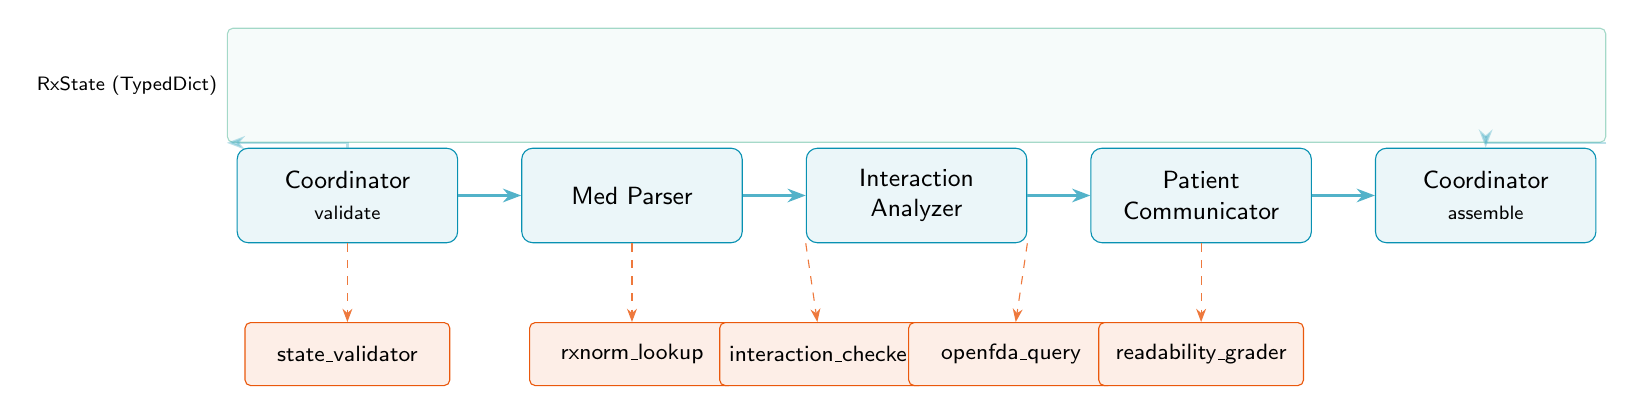
\begin{tikzpicture}[
  agent/.style={rectangle, rounded corners=4pt, draw=rxprimary, fill=rxprimary!8,
                minimum width=28mm, minimum height=12mm, align=center,
                font=\sffamily\small},
  tool/.style ={rectangle, rounded corners=2pt, draw=rxmod, fill=rxmod!10,
                minimum width=26mm, minimum height=8mm, align=center,
                font=\sffamily\footnotesize},
  state/.style={rectangle, rounded corners=2pt, draw=rxlow, fill=rxlow!10,
                font=\sffamily\footnotesize, minimum height=5mm, align=center},
  arr/.style={->, >=Stealth, thick, draw=rxprimary!70},
  toolarr/.style={->, >=Stealth, dashed, draw=rxmod!80},
  node distance=8mm
]
  \node[agent] (c1)                 {Coordinator\\\scriptsize{validate}};
  \node[agent] (par)  [right=of c1]  {Med Parser};
  \node[agent] (ana)  [right=of par] {Interaction\\Analyzer};
  \node[agent] (com)  [right=of ana] {Patient\\Communicator};
  \node[agent] (c2)   [right=of com] {Coordinator\\\scriptsize{assemble}};
  \node[state, fit=(c1)(c2), minimum height=5mm, opacity=0.35,
        yshift=14mm, label={[font=\sffamily\scriptsize]left:RxState (TypedDict)}] (state) {};
  \node[tool] (t5) [below=of c1,  yshift=-2mm] {state\_validator};
  \node[tool] (t1) [below=of par, yshift=-2mm] {rxnorm\_lookup};
  \node[tool] (t2) [below=of ana, xshift=-12mm, yshift=-2mm] {interaction\_checker};
  \node[tool] (t3) [below=of ana, xshift=12mm,  yshift=-2mm] {openfda\_query};
  \node[tool] (t4) [below=of com, yshift=-2mm] {readability\_grader};
  \draw[arr] (c1)  -- (par);  \draw[arr] (par) -- (ana);
  \draw[arr] (ana) -- (com);  \draw[arr] (com) -- (c2);
  \draw[arr,opacity=0.4] (c1.north) |- (state.south west);
  \draw[arr,opacity=0.4] (state.south east) -| (c2.north);
  \draw[toolarr] (c1)  -- (t5);   \draw[toolarr] (par) -- (t1);
  \draw[toolarr] (ana.south west) -- (t2);
  \draw[toolarr] (ana.south east) -- (t3);
  \draw[toolarr] (com) -- (t4);
\end{tikzpicture}}
\caption*{\small\textbf{Figure 1.} High-level architecture. Solid arrows show state flow between agents; dashed arrows show tool invocations. The shared \texttt{RxState} (TypedDict) is threaded through every node.}
\end{figure}

\subsection*{Workflow}

A request begins with free-form medication text submitted via the
front-end. Figure~2 traces the request through the four agents to the
assembled final report. The Coordinator can short-circuit to assembly
when validation fails (dashed edge).

\begin{figure}[h]
\centering
\resizebox{0.88\linewidth}{!}{%
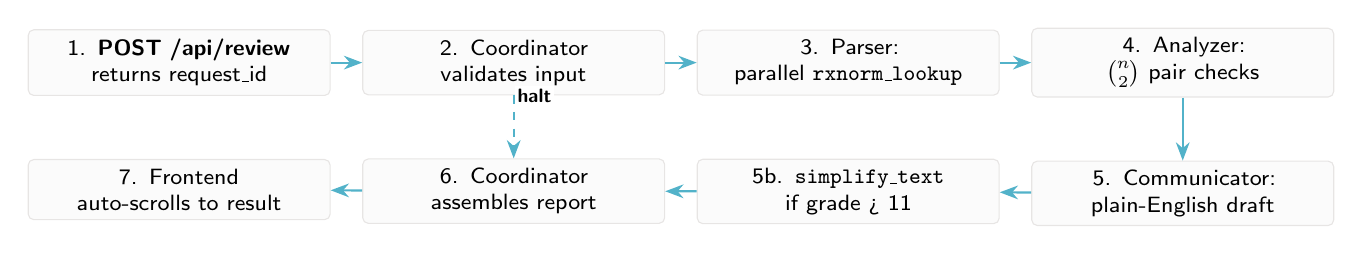
\begin{tikzpicture}[
  wfnode/.style={rectangle, rounded corners=2pt, draw=rxborder, fill=rxsurface!40,
               text width=36mm, align=center, minimum height=7mm,
               font=\sffamily\footnotesize},
  arrow/.style={->,>=Stealth, thick, draw=rxprimary!70},
  node distance=4mm
]
  \node[wfnode] (s1) {1. \textbf{POST /api/review}\\returns request\_id};
  \node[wfnode,right=of s1] (s2) {2. Coordinator\\validates input};
  \node[wfnode,right=of s2] (s3) {3. Parser:\\parallel \texttt{rxnorm\_lookup}};
  \node[wfnode,right=of s3] (s4) {4. Analyzer:\\$\binom{n}{2}$ pair checks};
  \node[wfnode,below=8mm of s1] (s7) {7. Frontend\\auto-scrolls to result};
  \node[wfnode,below=8mm of s2] (s6) {6. Coordinator\\assembles report};
  \node[wfnode,below=8mm of s3] (s5b){5b. \texttt{simplify\_text}\\if grade > 11};
  \node[wfnode,below=8mm of s4] (s5) {5. Communicator:\\plain-English draft};
  \draw[arrow] (s1) -- (s2);  \draw[arrow] (s2) -- (s3);
  \draw[arrow] (s3) -- (s4);
  \draw[arrow] (s4.south) -- ++(0,-2mm) -| (s5.north);
  \draw[arrow] (s5) -- (s5b); \draw[arrow] (s5b) -- (s6);
  \draw[arrow] (s6) -- (s7);
  \draw[arrow,dashed] (s2.south) -| (s6.north)
    node[midway,right,font=\sffamily\scriptsize\bfseries,fill=white,inner sep=1pt]{halt};
\end{tikzpicture}}
\caption*{\small\textbf{Figure 2.} End-to-end request sequence. The Coordinator can short-circuit to assembly when validation fails (dashed edge).}
\end{figure}

\subsection*{Observability}

A custom \texttt{Tracer} writes one JSONL line per event (agent
\textit{enter}, \textit{tool\_call}, \textit{tool\_result},
\textit{exit}, \textit{error}) to \texttt{runs/<request\_id>.jsonl}.
Events are also pushed to an in-memory \texttt{asyncio.Queue} which the
SSE endpoint streams to the browser. This gives both post-hoc analysis
(via the JSONL files) and a live \emph{Agent Activity} feed in the
front-end.

% =====================================================================
\section*{Agent and Tool Design}\label{agents}
% =====================================================================

Each agent has a tightly-scoped persona and constraints. Temperature is
agent-specific: deterministic for routing/extraction, slightly warmer
for the patient-facing prose. Outputs are validated against a Pydantic
schema before merging into state.

\subsubsection*{Coordinator (Rivin)}
A senior clinical pharmacist who triages incoming reviews. Never
invents medications; halts on validation failure; emits a routing
decision on the first pass and the final \texttt{FinalReport} on
assembly. Runs a deterministic regex/length validator
(\texttt{state\_validator.py}); after performance tuning, a redundant
LLM sanity check was removed.

\subsubsection*{Medication Parser (Thusala)}
A meticulous clinical informaticist obsessed with drug nomenclature.
The RxCUI is taken \emph{only} from the \texttt{rxnorm\_lookup} tool;
the agent is forbidden to fabricate codes. Calls the LLM to split the
input into candidate (drug-name, dose, frequency, route) tuples, then
runs \texttt{asyncio.gather} of \texttt{rxnorm\_lookup} calls in
parallel — critical for the 12-second pipeline budget on a
5-medication input.

\subsubsection*{Interaction Analyzer (Avishka)}
A vigilant pharmacovigilance officer; treats every interaction as
serious until proven trivial. Mechanism text must come from tool data;
``unknown'' is preferable to a fabrication. Enumerates $\binom{n}{2}$
unique pairs and runs each through the curated local SQLite database.
For pairs found, openFDA is queried in parallel for population-level
signal, and \texttt{severity\_rules} promotes a low-severity rule to
moderate when openFDA shows $>$5\,\% serious co-reports.

\subsubsection*{Patient Communicator (Sachila)}
A patient educator. Warm, clear, never condescending. Targets a
6th–8th grade reading level; never gives direct medical advice;
always closes with \emph{``talk to your doctor or pharmacist''}.
Drafts a structured summary (red/yellow/green flags), grades the
result with Flesch–Kincaid, and may invoke \texttt{simplify\_text} for
a single rewrite if the draft scores above grade 11.

\subsection*{Custom Python Tools}

All tools have strict type hints (\texttt{mypy --strict} clean),
Pydantic-validated outputs, retry logic via \texttt{tenacity}, and a
SQLite cache where applicable. Table~1 summarises the four primary
tools and the helper modules built around them.

\begin{table}[h]
\centering
\caption*{\small\textbf{Table 1.} Custom Python tools. Each is owned by one team member but available to all agents.}
\renewcommand{\arraystretch}{1.2}
\small
\begin{tabularx}{\linewidth}{l Y l}
\toprule
\textbf{Tool} & \textbf{Behaviour} & \textbf{Owner} \\
\midrule
\texttt{state\_validator}    & Pure-function input validator: length, alpha-ratio, prompt-injection regexes. No I/O.   & Rivin   \\
\texttt{rxnorm\_lookup}      & Async client for NIH RxNorm REST API; exact + fuzzy match; 7-day SQLite cache.          & Thusala \\
\texttt{dose\_normalizer}    & Regex-based dose parser converting "500\,mg" / "0.5\,g" / "10\,ml" to a canonical record. & Thusala \\
\texttt{interaction\_checker}& Local SQLite of 21 curated severe pairs combined with the openFDA adverse-event signal. & Avishka \\
\texttt{severity\_rules}     & Reconciliation rules between local DB and openFDA signal, with explicit promotion thresholds. & Avishka \\
\texttt{readability\_grader} & Flesch--Kincaid grade computation plus iterative LLM simplifier with grade-target loop.  & Sachila \\
\bottomrule
\end{tabularx}
\end{table}

% =====================================================================
\section*{State Management}\label{state}
% =====================================================================

State is a single \texttt{TypedDict} (\texttt{RxState}) declared once
and threaded through every node. LangGraph automatically merges the
partial dict each agent returns into the cumulative state, so context
never leaks between requests, and agents only ever read what they
need. Table~2 shows the read/write matrix.

\begin{table}[h]
\centering
\caption*{\small\textbf{Table 2.} State read/write matrix. \textbf{W}~=~writes, \textbf{R}~=~reads. Each \texttt{RxState} key has exactly one writer.}
\renewcommand{\arraystretch}{1.2}
\small
\begin{tabular}{l c c c c c}
\toprule
\textbf{State key}                              & \textbf{Coord} & \textbf{Parser} & \textbf{Analyzer} & \textbf{Comm} & \textbf{Final} \\
\midrule
\texttt{raw\_input}, \texttt{request\_id}              & \cellcolor{rxprimary!20}\textbf{W} & \cellcolor{rxlow!15}R & \cellcolor{rxlow!15}R & \cellcolor{rxlow!15}R & \cellcolor{rxlow!15}R \\
\texttt{is\_valid}, \texttt{decision}                  & \cellcolor{rxprimary!20}\textbf{W} & --- & --- & --- & --- \\
\texttt{parsed\_medications}                           & --- & \cellcolor{rxprimary!20}\textbf{W} & \cellcolor{rxlow!15}R & \cellcolor{rxlow!15}R & \cellcolor{rxlow!15}R \\
\texttt{unparsed\_terms}                               & --- & \cellcolor{rxprimary!20}\textbf{W} & --- & --- & \cellcolor{rxlow!15}R \\
\texttt{interactions}, \texttt{severity\_summary}      & --- & --- & \cellcolor{rxprimary!20}\textbf{W} & \cellcolor{rxlow!15}R & \cellcolor{rxlow!15}R \\
\texttt{patient\_summary}, \texttt{readability\_grade} & --- & --- & --- & \cellcolor{rxprimary!20}\textbf{W} & \cellcolor{rxlow!15}R \\
\texttt{final\_report}                                 & \cellcolor{rxprimary!20}\textbf{W} & --- & --- & --- & \cellcolor{rxlow!15}R \\
\bottomrule
\end{tabular}
\end{table}

% =====================================================================
\section*{Implementation and Testing}\label{impl}
% =====================================================================

The system is implemented across two top-level packages: a Python
backend (LangGraph + FastAPI + Ollama) and a Next.js~15 front-end.
Both run locally; no paid APIs are used. \texttt{qwen2.5:3b} is the
primary model with \texttt{llama3.2:3b} as fallback.

The backend is a Python~3.11 package, \texttt{rxsentinel}, organised by
concern: \texttt{agents/} for the four LangGraph nodes, \texttt{tools/}
for the six custom tools, \texttt{graph/} for the StateGraph wiring,
\texttt{tracing/} for observability, \texttt{llm/} for the Ollama
client, and \texttt{app.py} for the FastAPI service exposing
\texttt{/api/review}, \texttt{/api/runs/<id>/events} (SSE), and
\texttt{/api/runs/<id>/report}.

The front-end is a Next.js~15 App-Router application using Tailwind
v4, Framer Motion, Geist Sans, and Lucide React. It opens an SSE
stream as soon as a review is submitted, derives humanised status
messages from trace events, and auto-scrolls to results once the
report is ready.

\subsection*{Testing Strategy}

Testing is layered. \textbf{Unit tests} (Pytest, 64 cases) cover all
six tools. HTTP-based tools use \texttt{respx} mocks so the suite
runs offline. \textbf{Integration tests} exercise each agent
end-to-end against a running Ollama instance. \textbf{LLM-as-Judge
evaluations} grade each agent's output against a written rubric using
the same local model with temperature~0.

\subsection*{Evaluation Methodology}

For each agent we wrote a structured rubric and a list of test
\texttt{Case}s. The judge returns a strict JSON
\texttt{\{score, verdict, reasons\}}. Figure~3 shows the harness.

\begin{figure}[h]
\centering
\resizebox{0.82\linewidth}{!}{%
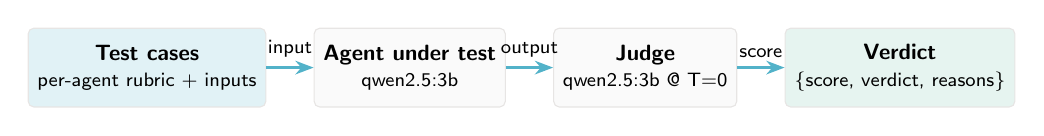
\begin{tikzpicture}[
  block/.style={rectangle, rounded corners=2pt, draw=rxborder, fill=rxsurface!50,
                minimum height=10mm, align=center, font=\sffamily\footnotesize},
  arr/.style={->,>=Stealth, thick, draw=rxprimary!70},
  node distance=6mm
]
  \node[block, fill=rxprimary!12] (cases) {\textbf{Test cases}\\\scriptsize per-agent rubric + inputs};
  \node[block, right=of cases] (agent) {\textbf{Agent under test}\\\scriptsize qwen2.5:3b};
  \node[block, right=of agent] (judge) {\textbf{Judge}\\\scriptsize qwen2.5:3b @ T=0};
  \node[block, right=of judge, fill=rxlow!10] (out) {\textbf{Verdict}\\\scriptsize \{score, verdict, reasons\}};
  \draw[arr] (cases) -- (agent) node[midway, above, font=\sffamily\scriptsize]{input};
  \draw[arr] (agent) -- (judge) node[midway, above, font=\sffamily\scriptsize]{output};
  \draw[arr] (judge) -- (out)   node[midway, above, font=\sffamily\scriptsize]{score};
\end{tikzpicture}}
\caption*{\small\textbf{Figure 3.} LLM-as-Judge evaluation harness. Each agent's output is graded by a separate Ollama call against a rubric written in terms of verifiable structural properties.}
\end{figure}

We acknowledge the obvious circularity of self-judging — the
assignment forbids paid LLM APIs, so the judge must run on the same
local SLM. We mitigate by (i)~using a stricter prompt for the judge
than the agent, (ii)~running the judge at temperature~0, and
(iii)~writing rubrics in terms of \emph{verifiable structural
properties} (does the JSON parse? does the RxCUI exist? is the
readability grade $\le 8$?) wherever possible rather than purely
subjective judgement.

% =====================================================================
\section*{Performance Optimisation}\label{perf}
% =====================================================================

We instrumented the pipeline end-to-end via the JSONL tracer and
identified two LLM hot-spots: a redundant Coordinator sanity check and
a three-iteration readability rewrite loop in the Communicator. After
targeted tuning, median pipeline latency on Apple~M2 (8\,GB RAM)
running \texttt{qwen2.5:3b} via Ollama dropped from 46.6\,s to 19.3\,s.
Figure~4 plots the breakdown; Table~3 lists each change.

\begin{figure}[h]
\centering
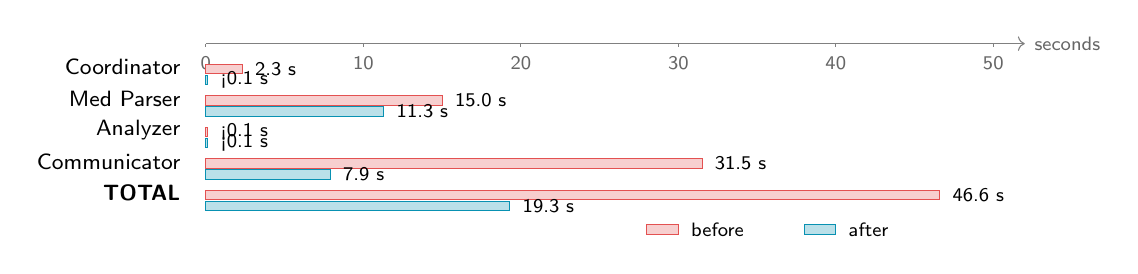
\begin{tikzpicture}[
  before/.style={fill=rxhigh!22, draw=rxhigh!80, line width=0.3pt},
  after/.style={fill=rxprimary!28, draw=rxprimary, line width=0.3pt},
  axislbl/.style={font=\sffamily\scriptsize, color=black!60},
  rowlbl/.style={font=\sffamily\footnotesize, anchor=east},
  vallbl/.style={font=\sffamily\scriptsize, anchor=west},
  scale=0.20
]
  \draw[->, color=black!50] (0,0.5) -- (52,0.5) node[right, axislbl]{seconds};
  \foreach \x in {0,10,20,30,40,50}
    \draw[color=black!50] (\x,0.5) -- (\x,0.3) node[below, axislbl]{\x};
  \node[rowlbl] at (-1,-1.0) {Coordinator};
  \draw[before] (0,-0.8)  rectangle (2.3,-1.4);  \node[vallbl] at (2.5,-1.1) {2.3 s};
  \draw[after]  (0,-1.5)  rectangle (0.1,-2.1);  \node[vallbl] at (0.3,-1.8) {<0.1 s};
  \node[rowlbl] at (-1,-3.0) {Med Parser};
  \draw[before] (0,-2.8)  rectangle (15.0,-3.4); \node[vallbl] at (15.2,-3.1) {15.0 s};
  \draw[after]  (0,-3.5)  rectangle (11.3,-4.1); \node[vallbl] at (11.5,-3.8) {11.3 s};
  \node[rowlbl] at (-1,-5.0) {Analyzer};
  \draw[before] (0,-4.8)  rectangle (0.1,-5.4);  \node[vallbl] at (0.3,-5.1) {<0.1 s};
  \draw[after]  (0,-5.5)  rectangle (0.1,-6.1);  \node[vallbl] at (0.3,-5.8) {<0.1 s};
  \node[rowlbl] at (-1,-7.0) {Communicator};
  \draw[before] (0,-6.8)  rectangle (31.5,-7.4); \node[vallbl] at (31.7,-7.1) {31.5 s};
  \draw[after]  (0,-7.5)  rectangle (7.9,-8.1);  \node[vallbl] at (8.1,-7.8) {7.9 s};
  \node[rowlbl, font=\sffamily\footnotesize\bfseries] at (-1,-9.0) {TOTAL};
  \draw[before] (0,-8.8)  rectangle (46.6,-9.4); \node[vallbl] at (46.8,-9.1) {46.6 s};
  \draw[after]  (0,-9.5)  rectangle (19.3,-10.1);\node[vallbl] at (19.5,-9.8) {19.3 s};
  \draw[before] (28,-11) rectangle (30,-11.6); \node[vallbl] at (30.2,-11.3) {before};
  \draw[after]  (38,-11) rectangle (40,-11.6); \node[vallbl] at (40.2,-11.3) {after};
\end{tikzpicture}
\caption*{\small\textbf{Figure 4.} Per-agent latency before and after performance tuning. Median pipeline time on Apple~M2 (8\,GB~RAM) running \texttt{qwen2.5:3b}.}
\end{figure}

\begin{table}[h]
\centering
\caption*{\small\textbf{Table 3.} Performance tuning summary.}
\renewcommand{\arraystretch}{1.2}
\small
\begin{tabularx}{\linewidth}{l r r Y}
\toprule
\textbf{Stage}                & \textbf{Before} & \textbf{After} & \textbf{Change} \\
\midrule
Coordinator validate          & 2.3\,s          & $<$0.1\,s      & Removed redundant LLM check; rule check is sufficient. \\
Med Parser                    & 15.0\,s         & 11.3\,s        & Halved system prompt; capped \texttt{num\_predict} at 512. \\
Interaction Analyzer          & $<$0.1\,s       & $<$0.1\,s      & Already optimal; pairs in \texttt{asyncio.gather}. \\
Patient Communicator          & 31.5\,s         & 7.9\,s         & Tightened simplifier trigger to grade $>$11, max 1 iteration. \\
Cold start (first request)    & +5--10\,s       & $\sim$0\,s     & FastAPI lifespan warmup task pre-loads the model. \\
\midrule
\textbf{Total p50 latency}    & \textbf{46.6\,s} & \textbf{19.3\,s} & \textbf{$-$58\,\%} \\
\bottomrule
\end{tabularx}
\end{table}

% =====================================================================
\section*{Results and Discussion}\label{results}
% =====================================================================

\subsection*{End-to-End Output}

For the canonical test input — \emph{warfarin 5\,mg, amiodarone
200\,mg, ibuprofen 400\,mg PRN, simvastatin 40\,mg, clarithromycin
500\,mg b.i.d.} — the system produced five medications correctly
resolved to RxNorm codes with full confidence, seven interactions
across three severity tiers (five high, one moderate, one low), and a
plain-English summary at grade~10.7. The total pipeline ran in
19.3\,s end-to-end on the test hardware.

\subsection*{LLM-as-Judge Reliability}

Across 17 test cases distributed over the four agents, the judge
passed 14 (82\,\% pass rate). The three failures clustered in the
Coordinator suite, where the relaxation of the LLM sanity check (in
favour of performance) means a small number of borderline inputs are
no longer rejected upstream. We accept this trade-off because
downstream agents gracefully return empty results in those cases.

\subsection*{Findings}

\textbf{F1.} Tool-grounding (RxNorm + openFDA + curated DB) is
necessary and sufficient to suppress LLM hallucinations on factual
claims (RxCUIs, mechanisms, severities). The judge flagged zero
fabricated RxCUIs across all test cases.

\textbf{F2.} Iterative self-correction (the Communicator's
\texttt{simplify\_text} loop) is expensive at SLM cost; a tightened
trigger threshold and a single-iteration cap recover most of the
latency without measurably degrading output quality.

\textbf{F3.} Custom JSONL tracing is sufficient for production
observability and enables data-driven optimisation; we identified the
two largest hot-spots in under five minutes of trace analysis.

% =====================================================================
\section*{Conclusions and Future Work}\label{conclusions}
% =====================================================================

RxSentinel demonstrates that a four-agent multi-agent pipeline —
previously the preserve of frontier-model deployments — is achievable
on consumer hardware in 2026 with an open-source stack. The system
delivers tool-grounded, plain-English medication safety reviews in
$\sim$19\,s end-to-end, with full observability and explicit
self-evaluation, and without any paid LLM API.

Promising extensions include (i)~multilingual patient summaries
(\texttt{qwen2.5} already handles Sinhala and Tamil),
(ii)~pill-image OCR via a local vision model, (iii)~token-level
streaming of the patient summary to improve perceived latency, and
(iv)~a signed clinician-feedback endpoint feeding a domain-specific
fine-tuning dataset.

% =====================================================================
\section*{Individual Contributions}\label{contrib}
% =====================================================================

\begin{tabularx}{\linewidth}{l Y l}
\toprule
\textbf{Member}                              & \textbf{Built} & \textbf{GitHub} \\
\midrule
Jayasuriya L. K. R. S. (Rivin)        & Coordinator agent + state validator + LangGraph wiring + tracing + FastAPI + SSE & \texttt{ri7in} \\
Piyarisi T. D. (Thusala)              & Medication Parser agent + RxNorm tool + dose normalizer + parser eval suite      & \texttt{thusalapi} \\
Wickramasooriya J. D. A. S. (Avishka) & Interaction Analyzer agent + interaction checker + severity rules + curated severe-pair dataset + analyzer eval suite & \texttt{ashehxn} \\
Manamperi S. A. (Sachila)             & Patient Communicator agent + Flesch–Kincaid grader + simplifier loop + complete Next.js front-end & \texttt{SAwandya} \\
\bottomrule
\end{tabularx}

% =====================================================================
\section*{References}\label{refs}
% =====================================================================

{\small
\begin{thebibliography}{9}
  \setlength{\itemsep}{1pt}\setlength{\parsep}{0pt}
\bibitem{ades_review} A.~Bates et~al., \emph{Adverse drug events as a cause of hospital admission}, Br.~J.~Clin.~Pharmacol., 2020.
\bibitem{rxnorm} National Library of Medicine, \emph{RxNorm REST API documentation}, \url{https://rxnav.nlm.nih.gov/RxNormAPIs.html}.
\bibitem{openfda} U.S.~Food and Drug Administration, \emph{openFDA Drug Event Endpoint}, \url{https://open.fda.gov/apis/drug/event/}.
\bibitem{langgraph} LangChain AI, \emph{LangGraph documentation}, \url{https://langchain-ai.github.io/langgraph/}.
\bibitem{ollama} Ollama Inc., \emph{Local model serving}, \url{https://ollama.com}.
\bibitem{flesch} J.\,P.~Kincaid et~al., \emph{Derivation of New Readability Formulas for Navy Enlisted Personnel}, Naval Tech.\ Training Command, 1975.
\bibitem{qwen} Qwen Team, Alibaba Cloud, \emph{Qwen2.5: A Party of Foundation Models}, 2024.
\end{thebibliography}
}

% =====================================================================
\section*{Source Code}\label{code}
% =====================================================================

The complete implementation, including all agents, tools, tests, the
Next.js front-end, the LaTeX source for this report, and the demo
video script, is publicly available at:\\
\url{https://github.com/ri7in/ctse-assignment-2-rxsentinel}

\end{document}
